\clearpage
\section{Platforma za razvoj igara Unity}

\subsection{MonoBehaviour i pisanje skripti u jeziku C\#}

\emph{MonoBehaviour} je osnovna klasa koju svaka Unity skripta nasle\v{dj}uje. Kada
koristimo C\# za skriptni jezik ovu klasu moramo eksplicitno da nasledimo \cite{unitydocs}. U svakom trenutku
mogu\'ce je isklju\v{c}iti ili ponovo uklju\v{c}iti skriptu. Isklju\v{c}ivanje
izuzima skriptu iz aktivnih skripti. Ukoliko je skripta uklju\v{c}ena i ima definisane
neke od specifi\v{c}nih funkcija koje se pozivaju u odre\dj enom trenutku tokom
\v{z}ivotnog ciklusa objekta smatra se aktivnom i reaguje na pozive tih funkcija
onako kako je korisnik to definisao. Neke od klju\v{c}nih funkcija su: \emph{Start()}, \emph{Update()},
\emph{FixedUpdate()}, \emph{OnEnable()}, \emph{OnDisable()}. \v{Z}ivotni ciklus skripte prikazan
je grafikonom ~\ref{fig:monoflowchart}. Kasnije u tekstu bi\'ce data preciznija obja\v{s}njenja
za najbitnije funkcije.

Drugim re\v{c}ima MonoBehaviour predstavlja definisano pona\v{s}anje nekog \v{z}ivog objekta
u svetu igre. Svaki objekat u svetu igre naziva se \emph{GameObject} i tipa je istoimene klase. Svaki
MonoBehaviour jeste \emph{GameObject}. Na GameObject je mogu\'ce dodati komponente. Treba imati 
na umu da ovakav sistem koji Unity pru\v{z}a nije pravi ECS (Entity Component System) te da zbog ovakvog
dizajna cela platforma radi sporije. Unity od skoro uvodi pravi ECS uz \emph{Burst Compiler}, ali ovo jo\v{s} uvek 
nije deo standardne platforme \cite{unitydocs}.

\begin{center}
    \begin{figure}
        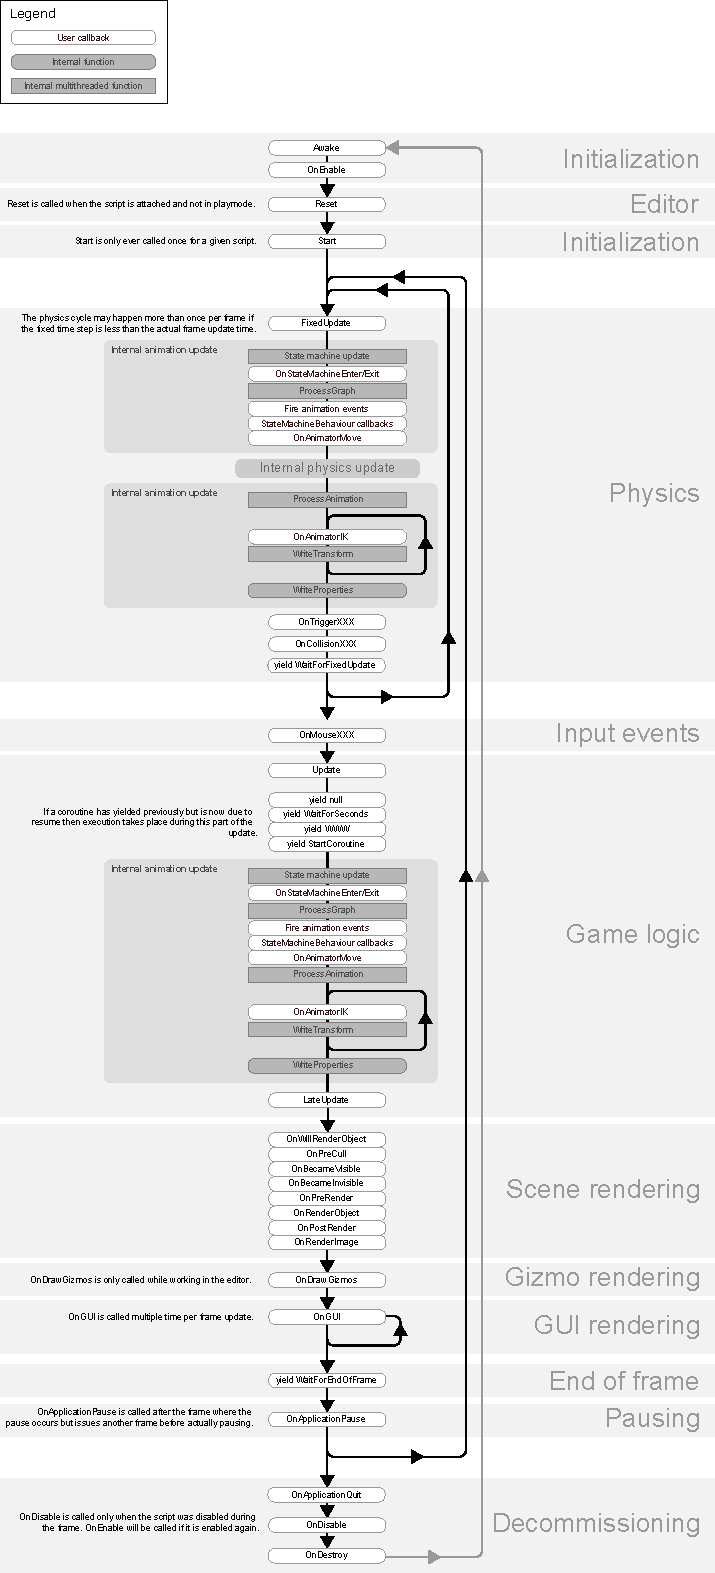
\includegraphics[width=0.7\textwidth]{Figures/mono_flowchart.pdf}
        \caption{MonoBehaviour lifecycle}
        \label{fig:monoflowchart}
    \end{figure}
\end{center}

\subsubsection{Scriptable Objects}
\label{sec:scriptobj}
\emph{ScriptableObject} je kontejner za skladi\v{s}tenje podataka, nezavisan od isntance klase. Oni omogu\'cavaju 
u\v{s}tedu memorije za podatke koji su konfigurabilni i ne menjaju se tokom izvr\v{s}avanja igre. Na primer, konfiguracije
poput ja\v{c}ine potiska, brzine okretanja i sli\v{c}no kod neprijateljskih brodova (kojih \'ce biti puno tokom igre).
Tako\dj e ono \v{s}to je zgodno jeste da te podatke mo\v{z}emo da sa\v{c}uvamo kao fajl u projektu, i onda jednostavnim
prevla\v{c}enjem u slot koristimo ~\ref{fig:scriptableslot}.

\begin{center}
    \begin{figure}
        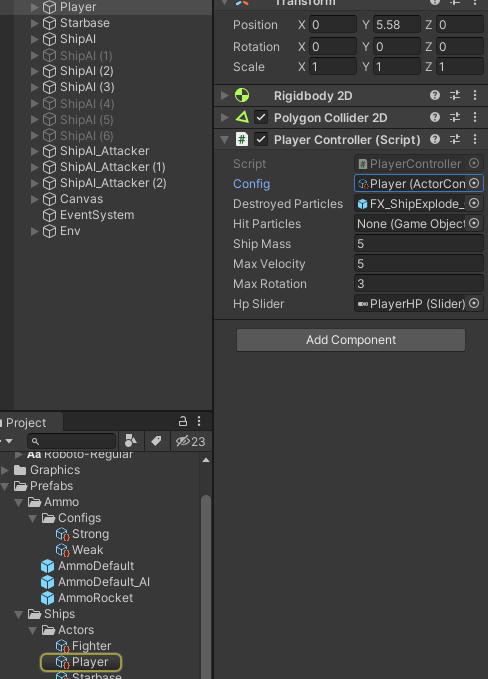
\includegraphics[width=1\textwidth]{Figures/ScriptableObjectSlot.png}
        \caption{Slot for scriptable object}
        \label{fig:scriptableslot}
    \end{figure}
\end{center}

\subsubsection{Coroutines}
\label{sec:coroutines}
Korutine su specijalne funkcije povratnog tipa \emph{IEnumerator} \v{c}ije izvr\v{s}avanje 
se mo\v{z}e pauzirati naredbom 

\begin{verbatim}
    yield return new WaitForSeconds(secs);

    // ili

    yield return null;
\end{verbatim}

gde ova druga pauzira izvr\v{s}avanje do slede\'ceg frejma. Korutine koristimo kada \v{z}elimo da se
neka stvar de\v{s}ava tokom nekoliko frejmova, recimo \v{z}elimo da napravimo odlaganje kraja igre nakon
uni\v{s}tenja svemirske baze (videti \ref{gamemanager}).

\subsection{Unity Editor}

Editor ~\ref{fig:unityeditor} je grafi\v{c}ko okru\v{z}enje namenjeno za postavljanje sveta igre. Editor
pru\v{z}a vizuelni pregled svih objekata na sceni, kamere i efekata. Prozor je podeljen
na nekoliko potprozora \v{c}ije uloge su da olak\v{s}aju pode\v{s}avnja i pregled igre.

\emph{SceneView} predstavlja pregled trenutne, aktivne scene. Scena predstavlja skup
objekata i kameru koji su u datom trenutku prikazani korisniku. Po\v{z}eljno je zasebne
logi\v{c}ke celine igre odvajati u zasebne scene, tako na primer, mo\v{z}emo imati scenu
za \emph{glavni meni} i \emph{scenu igre}, gde bi kroz u meniju bila omogu\'cena neka pode\v{s}avanja,
pregled najboljih rezultata i sli\v{c}no, dok je scena igre sama igra.

\emph{Hierarchy View} omogu\'cava pregled svih objekata na trenutnoj sceni. Objekti mogu
biti u roditelj-dete odnosu, te stoga i ime, jer tako \v{c}ine hijerarhiju.

\emph{Project View} daje pregled svih fajlova trenutno otvorenog projekta na disku.

\emph{Game View} obi\v{c}no slo\v{z}en pored pregleda scene prikazuje svet igre
onakav kakav \'ce biti prikazan igra\v{c}u, dakle bez pomo\'cnih elemenata poput 
kvadratne mre\v{z}e ili mogu\'cnosti pomeranja objekata. 

\begin{figure}[ht]
    \centerline{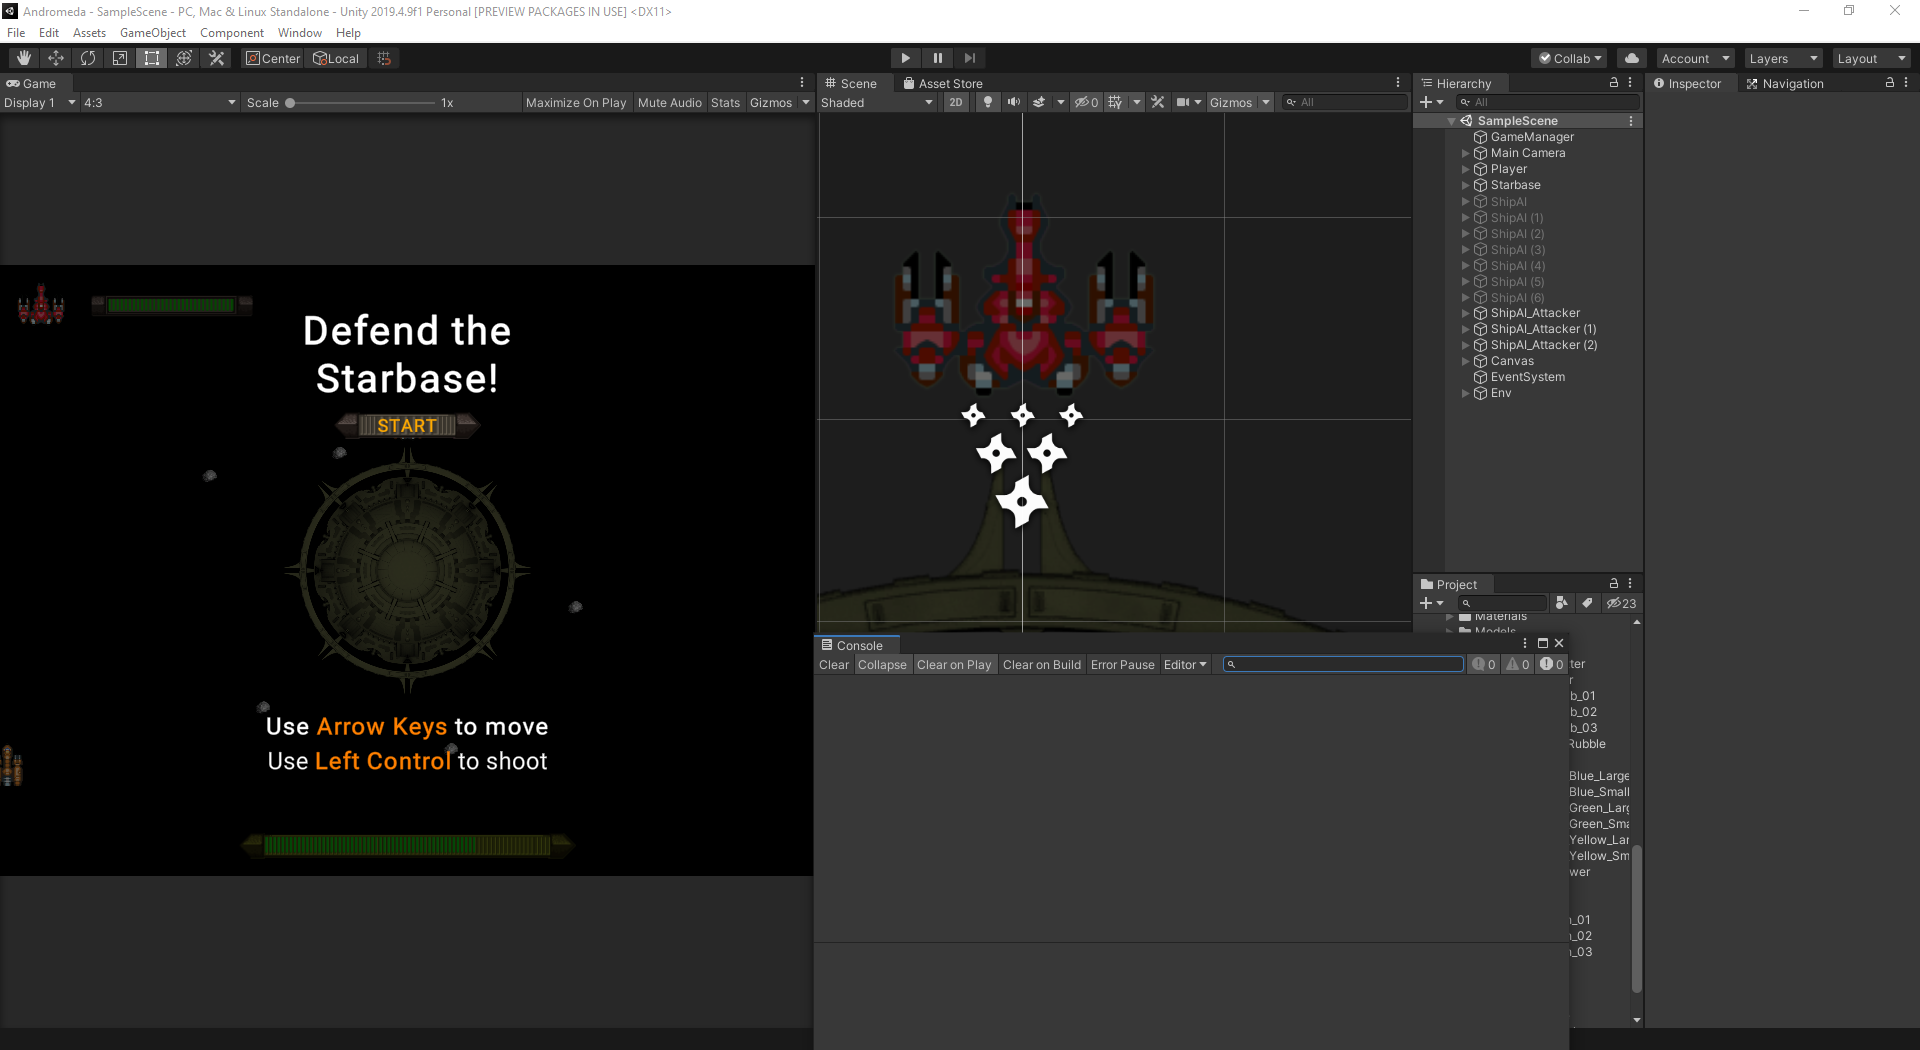
\includegraphics[width=0.9\paperwidth]{Figures/Editor.png}}
    \caption{Unity Editor}
    \label{fig:unityeditor}
\end{figure}

% \label{sec:Intro}
% ...

% \subsection{Exemplary Table}
% \label{subsec:Intro/table}
% ...

% \begin{longtable}{l|ccccc}
%   \caption{Exemplary Table}
%   \label{table:table-1}
%   \\
%   \textbf{Id} & \textbf{Col 1} & \textbf{Col 2}& \textbf{Col 3} & \textbf{Col 4} & \textbf{Col 5}\\
%   \hline
%   1 & Col 1 & Col 2 & Col 3 & Col 4 & Col 5\\
%   2 & Col 1 & Col 2 & Col 3 & Col 4 & Col 5\\
%   3 & Col 1 & Col 2 & Col 3 & Col 4 & Col 5\\
%   4 & Col 1 & Col 2 & Col 3 & Col 4 & Col 5\\
%   5 & Col 1 & Col 2 & Col 3 & Col 4 & Col 5\\
% \end{longtable}

% \subsection{Exemplary Section and Table Referencing}
% \label{subsec:Intro/rfs}

% See Table \ref{table:table-1} in Section \ref{subsec:Intro/table}  for details.